%------------------------------------------------
\section{Introducción} 
%------------------------------------------------

\subsection{Descripción}

\begin{frame}
	\frametitle{Descripción}
		\begin{block}{Motivación}
			\begin{itemize}
				\item Larga espera
				\item Optimización de el control del paso
			\end{itemize}
		\end{block}

		\begin{block}{Características generales}
			\begin{itemize}
				\item Control de tránsito vehicular y peatones
				\item Algoritmo flexible y manejo de prioridades según el contexto
				\item Implementado en FreeRTOS
				\item Semáforos de tres etapas
			\end{itemize}
		\end{block}
\end{frame}

\subsection{Glosario}

\begin{frame}
	\frametitle{Glosario}
	\begin{block}{Términos}
		\begin{itemize}
			\item Tramo: sentido en el que se circulan los vehículos
			\item Actividad: estado de un semáforo en el que el sensor del semáforo detecta vehículos o peatones
		\end{itemize}
	\end{block}
\end{frame}

%------------------------------------------------
\section{Especificación}
%------------------------------------------------

\subsection{Funcionamiento}

\begin{frame}
	\begin{columns}[T]
		\begin{column}{.35\textwidth}

			\begin{figure}[ht]
				\centering 
				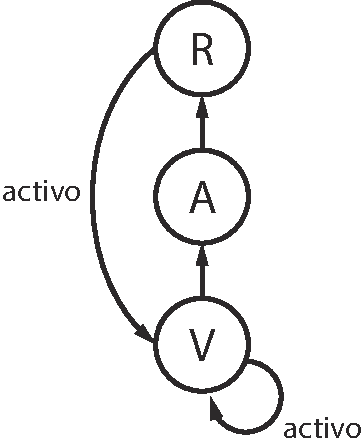
\includegraphics[scale=0.6]{diagramas/fsm-light.pdf}
			\end{figure}

		\end{column}
		\hfill
		\begin{column}{.65\textwidth}
			
			\begin{block}{Funcionamiento entre estados}
				\begin{itemize}
					\item Si el semáforo cambia de estado a activo, la transición es de rojo a verde
					\item Si solo el semáforo permanece activo y es el único, permaneces en verde
				\end{itemize}
			\end{block}
			\begin{block}{Funcionamiento entre semáforos}
				\begin{itemize}
					\item Los semáforos realizan Round-Robin entre todos si ninguno está activo
					\item Si al menos dos están activos se realiza Round-Robin entre los activos
					\item Si hay solo un semáforo activo, permanece en verde
				\end{itemize}
			\end{block}
		
		\end{column}
	\end{columns}
\end{frame}

%------------------------------------------------
\section{Problemas}
%------------------------------------------------

\subsection{Iteraciones}

\begin{frame}
	\begin{block}{Iteraciones}
		Aspectos más importantes en cada iteración
		\begin{itemize}
			\item[1] Conjuntos de activos y inactivos, fuerte pasaje de datos entre tareas,  difícil corrección, clases: sensor, controlador y semáforos
			\item[2] Con prioridades variables
			\item[3] Sin prioridades variables, simplificación del modelo.
		\end{itemize}
	\end{block}
\end{frame}

\subsection{Problemas con la implementación}

\begin{frame}
	\frametitle{Problemas con la implementación}
\end{frame}